\documentclass[12pt]{article}
\usepackage{sd}

\title{Stadium Traffic}
\team{13}
\addauthor{Parth Doshi;parthd@seas.upenn.edu}
\addauthor{Zain Mukaty;zmukaty@seas.upenn.edu}
\addauthor{Felipe Ochoa;felipeo@seas.upenn.edu}
\advisor{Dr. Andrew E. Huemmler;huemmler@seas.upenn.edu}
\reportname{Phase 2 Project Report}
\addbibresource{sources.bib}

\begin{document}
\maketitle
\abstract


Citizens Bank Park, the home stadium of the Philadelphia Phillies, is
located within city limits and is accessible by car, train and bus. In
the 81 home games of their 2012 season, the Phillies had an average
attendance of 44,021, for a total of over 3.5 million fan trips. All
these fans generate greenhouse gases traveling to and from the
stadium.

The Phillies have started the ``Red Goes Green'' initiative to reduce
their environmental impact by installing solar panels, planting trees,
and buying offsets for their carbon emmissions. They also offer tips
for fans who want to help with this mission.  No significant efforts
have been made so far, however, to quantify and reduce the
environmental footprint of these fans traveling to and from the
stadium.

This system meets two important needs that would help the Phillies and
their fans further reduce their carbon footprint.

First, it estimates the total amount of emissions currently generated
in based on the average distance traveled by fans and on the types of
transportation they use. These parameters are in turn estimated by a
comprehensive traffic model.

Second, the system provides fans information regarding alternative
travel options to and from the stadium by interfacing with the SEPTA
website. The tool is sensitive to the unusually-high demand placed on
transportation infrastructure around the game, and it gives fans
information on the congestion levels, travel time, and environmental
impact of each travel option.


\newpage

\tableofcontents

\newpage

\mainmatter

\section{Introduction}

\subsection{Overview}
Stadium Traffic aims to reduce the greenhouse gas (GHG) emissions from people going
to and from sports games. In particular, our project will focus on the
Philadelphia Eagles and Phillies stadiums.  We aim to build a model
that can be used to quantify the GHG emissions generated due to
people coming to and going from games. We will then develop solutions
to reduce the number of people coming by cars or leave over longer
time period and develop a traffic routing algorithm, aiming to reduce
the GHG emissions from idling cars waiting to leave the stadium. We
will test these on our model to find a successful combination. If we
can get the cooperation of Phillies/Eagles/Flyers and Philadelphia Police
Department, we hope to work with them to implement the results of our
project.

\subsection{Motivation}
All of us have been to large gatherings like
sports games, concerts or conferences and can therefore relate to the
traffic problems when everyone is trying to leave at the same time at
the end of the event. However, what most people don’t realize is the
environmental effect of this traffic. Our project aims to find
solutions to reduce this traffic and hence reduce the emissions while
cars idle in parking lots trying to leave.

The project is focusing on the Philadelphia Eagles, Phillies and Flyers
stadiums. Sports events draw huge crowds at peak traffic
hours and are therefore a great instance on which to model our
project. The Eagles are also undertaking a Go Green! initiative, which
is a push towards becoming more environmentally conscious. Some
initiatives that they have taken are the use of renewable energy
sources for their power consumption and using cups and plates made
from recycled materials. We believe that we can get the support of the
Eagles for our project, as it can be part of the Go Green! initiative
and further reduce the carbon footprint of the stadium.

When the football or baseball game ends, everyone tries to the leave
the stadium at the same time. Although traffic police conduct the
traffic, they do it in a haphazard way. Furthermore, the decision of
which gates to be open and which ones to remain closed is also done
using intuition rather than any efficiency-maximizing algorithm. We
saw this inefficient process as an opportunity to develop an algorithm
to reduce car idling time and GHG emissions.

\subsection{Project Goal and Objectives}
Although the overarching aim of our project is to reduce GHG
emissions due to people going to/from the sports games, we broke this
down into certain specific and measurable objectives:

\begin{enumerate}
    \item Develop a comprehensive model of transportation to and from
  the stadium.
    \item Quantify the total emissions due to transportation to/from
  games.
    \item Develop a tool to simulate the emissions impact of various
  initiatives to reduce private transportation usage (e.g. offering a
  discounted drink to someone who rides the SEPTA).
    \item Create an algorithm to optimally route exiting vehicle traffic
  according to total emissions generated.
    \item Develop a method for the Philadelphia traffic police to
  implement the traffic routing recommendations of our project.
\end{enumerate}

The success of each of the objectives can be measured and how we would
measure the success is stated below:

We would consider a success model one that takes inputs such as trip
distribution, number of attendees, start and end time and produces
outputs such as average idling time and number of cars.

The aim of the project is to reduce GHG emissions, so we need to be
able to measure and quantify GHG emissions from idling cars.

Our model should be able to quantify the effect of different
incentives on GHG emissions so that we can test different
strategies and find the optimal combination.

Optimal routing of traffic can impact GHG emissions from idling
cars, so we need to create an algorithm that can be constraint
optimized. A working algorithm can help the traffic police conduct
traffic in a more organized manner.

Having a front-end system that can be used by the Philadelphia Police
will allow our algorithm to be implemented and hence allow our project
to have an impact. Therefore we need a mock-up of a computer or phone application
that can be used by the police while conducting traffic.

\subsection{Constraints}
The main constraint is the cooperation of the Philadelphia
Eagles/Phillies/Flyers and Philadelphia Police Department because without
their cooperation we cannot implement our project. However, our
advisor Dr. Huemmler has good relationships with both sets of organizations
and has been trying to get their support for the project.

Another constraint is the team’s lack of experience with
transportation engineering.  Since the project involves the
understanding, modeling and optimizing of transport systems, this
would be a constraint. However, we have taken an initiative to get the
help of Professor Vukan Vuchic, a senior professor in transport
engineering, and began familiarizing ourselves with relevant transport
systems concepts under his guidance.

Finally, our last constraint is the data collection required to build
a representative model. However, we have been trying to get the
required information from the Eagles, Phillies, Flyers and other government
departments.



\section{Discussion of Previous Work}


\subsection{Scholarly Work}
Scholarly research in transportation model distinguishes between two
broad approaches: \cite{kitamura1988}

\begin{description}[style=nextline]
    \item[Activity-based] Modeled at the individual level. Considers
  trips arising from different activities that comprise a tour. (E.g.,
  travel to kids' school, then to work, then to the grocery store, and
  finally back home). \cite{kitamura1988}
    \item[Trip-based] Modeled at the Traffic Analysis Zone (TAZ)
  level. Considers broader characteristics such as demographics of a
  neighborhood to model trip times and volumes.\cite{murthy01}
\end{description}

The activity-based model dominates in the most recent academic
literature, but from our survey, the trip-based model still appears to
be the most frequently used type of model by government
agencies. Within the trip-based models the dominant kind appears to be
the four-stage model, which breaks down into four components:
\cite{murthy01}

\begin{enumerate}
    \item Trip Generation
    \item Trip Distribution
    \item Mode Choice
    \item Trip Assignment
\end{enumerate}

In all the applications saw, each of those stages is further refined
by the category of the trip being modeled. The usual breakdown is:

\begin{description}
  \item[Home-based work] (HBW) Trips from home to work or vice versa.
  \item[Home-based shop] (HBS) Trips from home to go shopping and back
(sometimes omitted).
  \item[Home-based other](HBO) Other trips having the home as an
origin or destination.
  \item[Non-home-based work] (NHW) Trips to or from work not in HBWl
  \item[Non-home-based other](NHO) All other kinds of trips.
\end{description}

One of the main benefits of the trip-based approach is its long
history and current widespread use. The model is also readily
modularized, and was easily adapted and specialized for our
purposes. On the other hand, it is more simplistic than the
activity-based model, since it ignores the interactions of past trips
generated on future trip generation. The activity-based model,
however, has a clear computational disadvantage. The level of detail
the model reaches means that it is very demanding computationally, and
is also hard to break into subcomponents.

Our approach combined aspects from both styles (as detailed in section
3), but borrowing the terminology of the trip-based style.

\subsubsection{Phoenix, Arizona Planning Authority}
In 2011 the planning authority in Phoenix, Arizona, MAG, undertook an
extensive project to model transit movement to planned special events
in the region. \cite{kuppam11} Our chosen topic, sports games, falls
under their category of a planned special event. The authors identify
the proportion of special events patrons who utilized light rail
v. alternative modes of transportation and their approach to modeling
demand and modal choice for this event. While the results are specific
to their application, the methodology helped inform our own approach.
focus.

\subsubsection{Robertson Stadium}
Gunda Corporation performed a relatively similar project to the one we
developed for Robertson Stadium at the University of
Houston.\cite{gunda} Although the stadium has a lower capacity than
the Phillies stadium, \cite{robertson-stadium} it is home to an MLS
team, and has to abide by all the traffic management principles of a
professional sports team. The scope and aim of Gunda's analysis
differed from our own, but their analysis helped guide our design of
a component of our model. (The micro-car module, see section 3)

\subsection{Time-Expanded Graphs}
Much of our work on the SEPTA model, discussed in section 3, was
informed by the work of Frank Schulz in his
dissertation\cite{schulz2005timetable}. The timetable routing problem
is a special class of traffic assignment problem in which time is
naturally discretized (by the timetable). Because of this special
structure, these problems don't need to rely on the inaccurate or
computationally expensive algorithms that discretize time. Instead,
the \emph{time-expanded graph} refers to a graph where nodes
correspond to moments in time at a particular location (e.g., Grand
Central at 3:15pm). Edges correspond to direct transit lines between
two space-time locations.

Although we did not venture into the more sophisticated algorithms
described in \cite{kohler2002time}, the discussion about their
computational efficiency helped us make certain design choices
discussed in section 3. Also of use in this regard were
\cite{xuan2003computing} and \cite{george2008time}.


\subsection{Queue-Based Modeling}
Our work on the micro car model, also discussed in section 3, took a
completely different approach to that of the SEPTA model. The
queue-based approach that we used is described in great detail in
\cite{van2007modeling}. As described by Van Woensel and Vandaele,
queueing models are primarily used to model individual intersections,
as in \cite{ruskin2002modeling} or \cite{kyte2009validating}. These
queueing models operate by considering car arrivals as a stochastic
process with a single server at the intersection. The focus of these
types of models is more on the interaction of multiple cars at an
intersection, like in \cite{prasetijo2012capacity}.

Our model differed in two important ways from those mentioned above

\begin{enumerate}
    \item All the cars in the stadium parking lot are headed in the
  same direction: \emph{out}
    \item The parking lot we considered has over 100 nodes
\end{enumerate}

\subsection{Dynamic Traffic Assignment}
When specialized to cars, the assignment problem can be solved in a
variety of ways. One particularly high-level distinction is between
static and dynamic assignment, which can be thought of roughly as the
difference between the steady-state and the transient solution to the
problem. The algorithm we developed had at its core the ideas
developed by Dial \cite{dial2006path} and Nie
\cite{nie2010class}. They describe a class of algorithms to
efficiently solve the dynamic traffic assignment problem and a metric
called user equilibrium (UE) to measure the effectiveness of these
algorithms. Boyce \cite{boyce2003convergence} has an extended
discussion of user equilibrium.

\subsection{Group Members' Prior Work}
One of our group members had had experience working with Penn Transit
to improve the dispatching efficiency of their bus operations around
campus. This work allowed for in-depth understanding of queuing theory
and demand generation, which was extremely useful in our micro car
module, described in more detail in section 3. Using elements of the
prior project, combined with additional concepts from traffic
engineering, we developed an accurate model.



\section{Strategic Plan/Structure}

The driving principle behind our strategic plan can be summarized as
``Benchmark, then improve.'' We are analyzing a real-world system
(that of fans traveling to and form the stadium), and we are building
our own software system to simulate it. Our project will therefore
first focus on computing `sensible' emissions values for an average
game, and will then develop a full software model to quantify the
impact of different policies that could be put in place. In
engineering terms, we are first calculating the equilibrium or
``trim'' condition and then we will focus on disturbances away from
it.

\subsection{System Proposed Approach}
The approach to both problems will of necessity be similar, and our
aim is to design our solution to the first problem with a great deal
of flexibility so that it may be readily adapted for use in the second
phase of the project. Our phase 1 model will have five main components
that correspond to the four steps of the UTMS plus a GHG
calculator. The blocks described below correspond to the block diagram
shown in figure \ref{mainsystem1}.

\begin{figure}[htp]
  \centering
  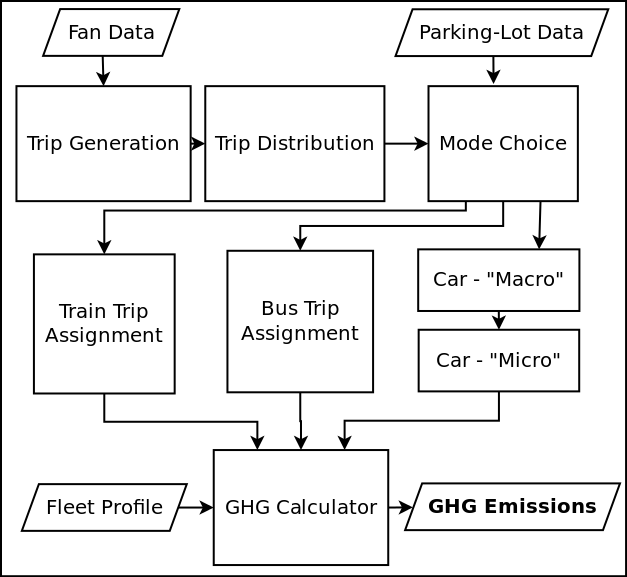
\includegraphics[height=8cm]{graphics/fullsystem1.png}
  \caption{System block diagram of our phase 1 model}
  \label{mainsystem1}
\end{figure}

\begin{description}[style=nextline]
    \item[Trip Generation] We will need to gather data on the
  geographic distribution of the fans that attend the games. We hope
  to obtain a good amount of data from the Eagles to aid in this
  section. Absent that data, we will have to resort to theoretical
  models commonly used in the industry, such as the Gravity Model. We
  will also be gathering data on timing of the trips, either through
  direct observation, or ideally from already existing records.
    \item[Trip Distribution] This step in the modeling is
  straightforward, since we know that fans are traveling to and from
  the stadium (or a nearby parking lot).
    \item[Mode Choice] This phase involves matching each trip in the
  database to a mode of travel (i.e. Car vs. SEPTA vs. Bus). We plan
  on using parking-lot data to estimate car use, and, if possible, get
  station-level information directly from SEPTA. A variety of
  theoretical models exist to help validate the gathered data.
    \item[Trip Assignment] Is the selection of the specific lines,
  streets, highways, and stations that each trip will follow. At this
  stage, we will break the model into subsystems for each of the
  possible means of transportation.
    \begin{description}[style=nextline]
        \item[Trains] A great deal of information is available on the
      website regarding lines and schedules that we have used to build
      a software representation of the network. With some
      well-established linear optimization algorithms, we will be able
      to model the exact path taken for every trip assigned to SEPTA
      trains. A preliminary step is to populate the station model, as
      shown in figure \ref{septa-db}. Then, we will use established
      algorithms to run the model based on this database, as shown in
      figure \ref{septa}
        \item[Buses] Schedules and stops are also available at
      www.septa.org. We will merge this database with the
      information available on Google Maps to obtain location data.
      There are also well-established algorithms we can use to model
      the paths of every trip.
        \item[Cars] Our car model will be split in two: \label{cars}
      \begin{itemize}
          \item At a "micro" level, we will model the road network in
        and around the stadium parking lot based on existing databases
        complemented with hand-input data that we extract from maps
        and planning documents. This portion will be used to model the
        exiting cars, since we believe the congestion at the end of a
        game results in substantial GHG emissions.
          \item At a "macro" level, we will use the same TAZs as in
        the trip generation phase, and calculate a sample path to the
        stadium based on highways and main roads.  We will have to
        encode the network of such roads and use our own algorithms.
        Alternatively, depending on the resulting number of TAZs, and
        subject to special authorization, we could use the Google Maps
        API to programmatically retrieve routing information.
      \end{itemize}
    \end{description}
      \item[GHG Calculator] This subsystem will be a memoryless
    function mapping a trip to an estimated emissions value. Our
    preliminary assumption is that trips taken on public transit
    contribute no additional GHG, since we are taking the bus and
    train schedules as given. For cars, there are a multitude of
    published methods for estimating emissions. We will have to
    estimate a fleet profile (average age and size) to use one of
    these models. We expect that it will be a function of total
    highway distance/time, local street distance/time, and idling
    time. When properly built, the output from this subsystem will be
    our first main deliverable.
\end{description}

\begin{figure}[htp]
  \centering
  \begin{subfigure}{.504\textwidth}
    \centering
    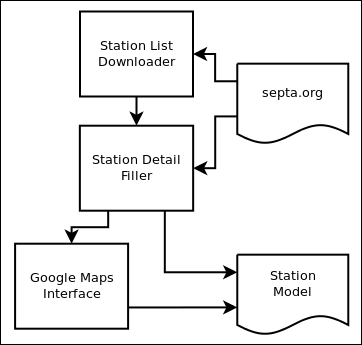
\includegraphics[width=\textwidth]{graphics/septa-db.png}
    \caption{Populating the station database}
    \label{septa-db}
  \end{subfigure}
    \begin{subfigure}{.394\textwidth}
    \centering
    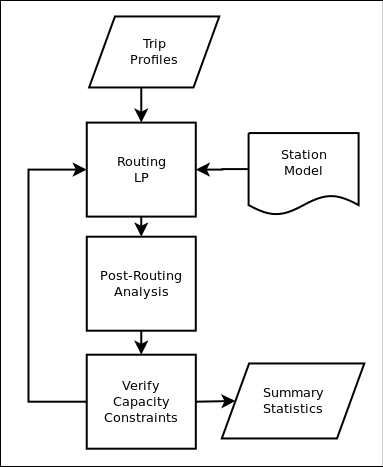
\includegraphics[width=\textwidth]{graphics/septa.png}
    \caption{Operation of the train subsystem}
    \label{septa}
  \end{subfigure}
  \caption{Components of the SEPTA Train Model}
% septa.png 383 w x 467 h
% septa-db.png 362 w x 345 h
% w1 * 467 / 383 = w2 * 345 / 362
% w2 = w1 * (467 * 362) / (383 * 345) = w1 * 1.2794
% w1 + w2 = .9\textwidth
% w1 = .9\textwidth / ( 2.27924)
%    = .394\textwidth
% w2 = .504\textwidth
\end{figure}

For the second phase of the project, as mentioned above, we will seek
to leverage as much of the modeling work from phase one as
possible. The goal for this phase will be to focus on converting the
existing model into a usable simulator. A key objective will be
incorporating a variety of inter-system feedback mechanisms that will
allow for a more accurate model.  The degree of detail in these
feedbacks mechanism will be constrained by the computational
complexity of including them (see Table \ref{specs} for computational
requirements) and by the design constraints of our subsystems (see
Section \ref{requirements}) Since there may be limited opportunities
to validate our model (until the next season begins), a key
performance metric will be the consistency of results, which in
technical terms, means that the system should reject small
disturbances in the inputs.  Conceptually, changing the base fare for
SEPTA or increasing the cost of parking by small amounts should not
result in wildly different behavior. This sensitivity will be a key
measure we will use in determining the right level of complexity to
build into the model.

Some examples of feedback mechanisms we are considering at this stage
are:

\begin{description}[style=nextline]
    \item[Congestion] If a fan spends 45 minutes stuck in the parking
  lot unable to move, we expect that fan to be more likely to take the
  train for the next game. A more detailed discussion of the fan model
  lies below.
    \item[Scheduling] If SEPTA notices trains traveling fuller on game
  days, they may choose to alter schedules in the future.
    \item[Uncertainty Effects] As fans try different modes of
  transportation, they may refine their predictions of travel times
  and convenience.
    \item[Fleet Composition] We suspect the fans that are most likely
  to start using public transit may have cars with above-average fuel
  efficiency, whereas the fans that take their trucks to tail-gate
  parties will likely continue to use their less-efficient cars.
  These effects would alter the fleet profile and hence average
  emissions calculations.
\end{description}

Regardless of what feedback loops we ultimately incorporate, we will
have to build a model of the fans' utilities, to capture the effects
of the various incentive schemes on trip generation profiles. At this
stage we expect we will be using an agent-based technique for this
subsystem, which will have as inputs the TAZs and some demographic
data. Cooperation from the Eagles will be important in fine-tuning
this part of the model.

The expanded model can be seen in the block diagram in figure
\ref{mainsystem2}. We have included the incentive structure as an
input in the diagram. We expect to make a GUI for this input to the
model, which will have a variety of options. For now, we have left
these unspecified as we will have to discuss with the Eagles what
their interests are. The other block added is the preference model,
which will be an agent- or automata-based model about fan preferences,
i.e. how they value travel time, convenience, comfort, and other
parameters that differ between the different modes of transportation.

\begin{figure}[htp]
  \centering
  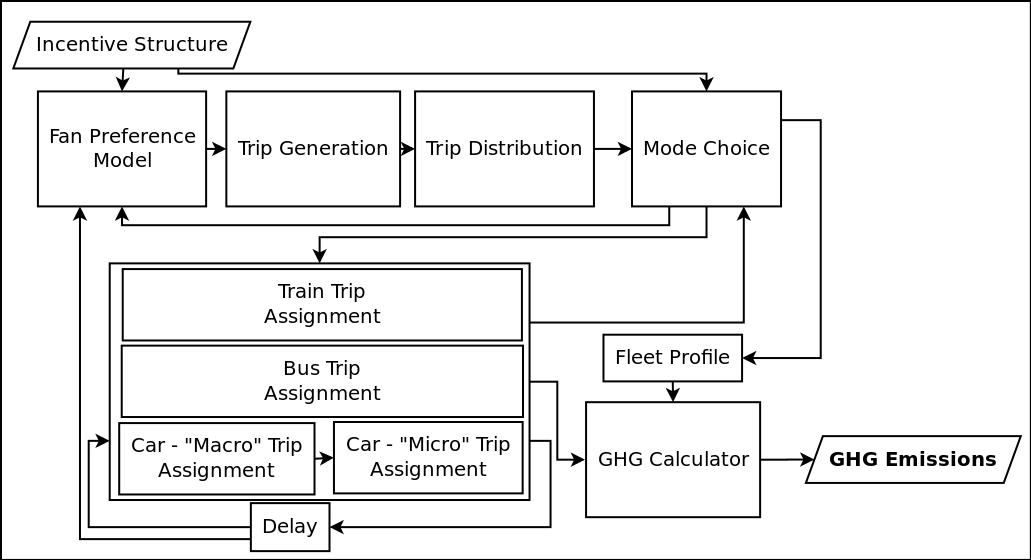
\includegraphics[height=8cm]{graphics/fullsystem2.png}
  \caption{Full system incorporating feedback}
  \label{mainsystem2}
\end{figure}

\subsection{System Specification}
Our end system must have a GUI that can be used by Eagles management
to input proposed incentives and that will output the projected change
in GHG. The input must be intuitive and friendly enough that it does
not require a manual for a user of average computer literacy to learn
to use it in 10 minutes or less. Additionally, once a user is familiar
with the interface, varying parameters on a proposed incentive program
should not require more than 2 minutes of the user's time.

The back-end must be flexible and have a documented API so that a
software developer may write extensions to the model (e.g. different
incentive types) or refine sub modules (e.g. a more efficient traffic
assignment subsystem) without having to modify the other components of
the software. Additionally, the model must be fast enough so that
initial estimates of GHG emissions under certain incentive schemes may
be computed within 5 minutes. In addition, detailed logs and reports
(e.g. emissions over time graphs) should be accessible to a more
knowledgeable user through the same GUI.

The program must handle improper input robustly and must be able to
deal with exceptions and errors gracefully. Specifically, a user of
average computer literacy should be able to understand error messages,
and, in a worst-case scenario, should be able to simply reset the
application to restore functionality.

The subsystem specifications are laid out in table \ref{specs}
\begin{table}[htp]
  \newlength\midcolumnwidth
  \midcolumnwidth=.74\textwidth plus 10\tabcolsep minus 10\tabcolsep
  \centering
  \caption{Specifications table}
  \label{specs}
  \begin{tabular}{%
    >{\raggedright}p{.11\textwidth}%
    p{\midcolumnwidth}%
    >{\raggedright\arraybackslash}p{.15\textwidth}}
  \firsthline
  \bfseries Module & \bfseries Qualitative Requirements & \bfseries
  Quantitative Performance Requirements \\ \hline
  Trip Generation & Interface with a database of TAZs and (if
  possible) a database of sanitized user data in strict XML format.
  Output a list of trips specifying the origin and time of each one. &
  $5\,s$ per $50,000$ trips \\
  Trip Distribution & Pass through the list from the trip generation
  module. & N/A \\
  Mode Choice & Read in sanitized parking-lot data in SQL,
  station-level usage information, and TAZ demographic profiles.
  Assign a mode choice to each entry in the the list from the trip
  distribution module.
  Output a vector of the different trips in each category and
  summary statistics for each mode (e.g. utilization percentage). &
  $10\, s$ per $50,000$ trips \\
  Trains & Read in a line and schedule XML database
  and accept an input of trip origin and time pairs. Calculate the
  most direct path to the stadium for each trip , subject to capacity
  constraints. Output summary statistics and trip list. & $1\,$min
  per 50,000 trips \\
  Buses & As above, with its own (larger) database. The trip profiles
  must not specify stop-by-stop, but rather total distance, to
  within 5\% error. & $1\,$min per 50,000 trips \\
  Cars & (See below) & $1\,$min per 50,000 trips total \\
  Cars - Micro & Accept the list of trips and read in a database of
  the road network in and around the stadium. Compute total distance
  and idling time per car to reach the highways/main roads. & \\
  Cars - Macro & Accept the same list of trips as above and compute
  total highway and secondary road times across all trips. Optionally
  interface with the Google Maps API. & \\
  GHG Calculator & Process the outputs from the trip assignment
  modules and compute an overall level of GHG emissions. & $10\,s$
  per 50,000 trips \\
  \lasthline
  \end{tabular}
\end{table}
\subsection{Hardware and Software Requirements}
\subsubsection{Hardware Requirements and Design Approach}
The hardware requirements for this project will feature towards the
tail end of the project.  The end-user (be it the Eagles/Phillies or
the policemen directing traffic), will be receiving a finished piece of
software from us, which would require specialized hardware to deal
with it.

In order to make the software/algorithm we create generalizable, we
will be utilizing a popular hardware choice of either a personal
computer or a portable device (iOS/Android). The choice will be made
upon further discussion with the Eagles and at this time we are unable
to provide reasons for a technical hardware choice.

\subsubsection{ Software Requirements and Design Approach}
The software we create will be created primarily in Matlab and
Python. The requirements we have from our software will be as follows:
\label{requirements}
\begin{description}[style=nextline]
    \item[Modularity] We should we able to switch out one
  implementation of the train model, for instance, and replace it
  seamlessly with another, more efficient implementation.
    \item[Scalability] It should be able to handle a large number of
  inputs and not break under scale. It will have to deal with tens of
  thousands of fans inhabiting the model.
    \item[User-Friendliness] We want the final output, or GUI, to be
  extremely user-friendly and it should be operational without a
  manual.
\end{description}

We expect to use commonly available hardware. In summary, we will be
looking to create a model that takes in data about demand generation
and incentives and uses that to determine the modal usage of
transportation to Eagles games.  Finally, we will be using the model
to determine the amount of time cars idle and based on expected CO2
emission rates, we will be determining the impact of the incentives
inputted into the model. We will also be developing a module to
incorporate feedback, allowing for ``state'' in our model (i.e. prior
experiences impact future choices).


\subsection{Test and Demonstration}

%\subsubsection{Test}
%\subsubsection{Demonstration}
\input{includes/tests_and_demo.tex}

\subsection{Schedule}

The schedule consisted of the different tasks that we estimated we
would need to accomplish in order to have a successful project. The
tasks can be broken into

\begin{itemize}
  \item Planning and design
  \item Creating the required subsystems
  \item Integrating the subsystems into one system
  \item Testing and validation
\end{itemize}

Each task was assigned to only one individual although others may also
have been working on the task, but the assigned individual was
accountable to get it done correctly and on time. Based on the Gantt
chart and schedule it is clear that we aimed to work consistently over
the course of the year, including winter break, to meet the milestones
(course requirements) and not fall behind schedule. Although there
were delays in completing some tasks, we did not let that disrupt our
uniform workflow by reallocating resources to other tasks and either
getting them started early or completed faster by having more people
working on it.

The main challenge that we faced was the delay and inability to
establish contact with the Philadelphia Phillies or Philadelphia
Police Department. The lack of contact had lead us to postpone some of
our earlier tasks till we met them to understand their requirements
and get the required data from them. Our advisor, Dr. Huemmler, worked
very hard to try to get us in contact with them and sent multiple
emails and even letters on official University of Pennsylvania SEAS
letterhead to five people at the Phillies and Police department, but
still did not manage to schedule a meeting.

Finally, during mid March, we reached our deadline to determine the
end users and had to disregard the Phillies and make the sports fans
the end users. This lead two major consequences for the schedule:

\begin{enumerate}
  \item Changing some of the originally scheduled tasks
  \item Non-uniform distribution of work
\end{enumerate}

Since the end users changed, there were certain aspects of the system
that needed to be removed and other subsystems and functionalities
that had to be added to accommodate the change in requirements. The
Incentive Scheme or Tailgate Model had to be removed because now we no
longer had to determine the effect of various incentive schemes on
trip distribution or modal distribution. However, we had to develop a
website for the front end that synthesized the information from the
simulation and GHG (Green House Gas) Emissions model. We also had to
increase the scope of the SEPTA model to incorporate the entire SEPTA
system rather than just the station level model for AT\&T
Station. Finally, we had to incorporate travel time into both the
SEPTA and Car models because that would be an important output for the
end user.

Due to this major change when there was approximately one month
remaining before demo day, there was a lot of work that needed to be
done and we had to allocate more time to the project that we had
originally scheduled. However, we were able to do this for two main
reasons. Firstly, we had anticipated this and as accordingly set a
contingency plan, which involved pushing some tasks back that were the
same for both systems, and pushing other tasks forward that were
specific to either one of the systems. Secondly, when we were
originally making the schedule we had kept slack time in the
tasks. There was a third unanticipated factor of over-estimating the
time it would take to complete certain tasks, which helped us at the
end. We had over-estimated the time it would take to make the SEPTA
subsystem and GHG Emissions model, however, the time we had saved in
making the model originally, we spent on updating it to suit the new
requirements. However, developing the new front-end system took a lot
of time and lead to greater than proportionate time spent on the
project in April.

Despite the late scheduling changes, we managed to have a working
model and front-end website by demo day. However, if we were to do
this again we would have set the deadline to determine the end user to
a much earlier date, such as the end of first semester. This would
have given us more time to refine the front-end and even launch the
website before demo day in order to get user feedback and incorporate
that into our model. However, we used alternative methods of testing
and validation.



\section{Results}


\subsection{Trip Generation}

We had to rely on the Gravity Model of transportation planning in
order to estimate the trip generation. However, we adjusted it to fit
our needs. Since the end point of all trips was the same, we did not
need the factor of $P_j$ and the model constant $K$ was just a
normalizing factor to make the total number of trips from all zones
equal to the total attendance. $K$ was calculated as
$(T_{ij}/T_{total}) \times (\mathrm{Total attendance})$. The map below
shows the results of the Gravity Model by displaying the number of
trips originating from each zip code to the stadium.

\begin{figure}[htp]
  \centering
  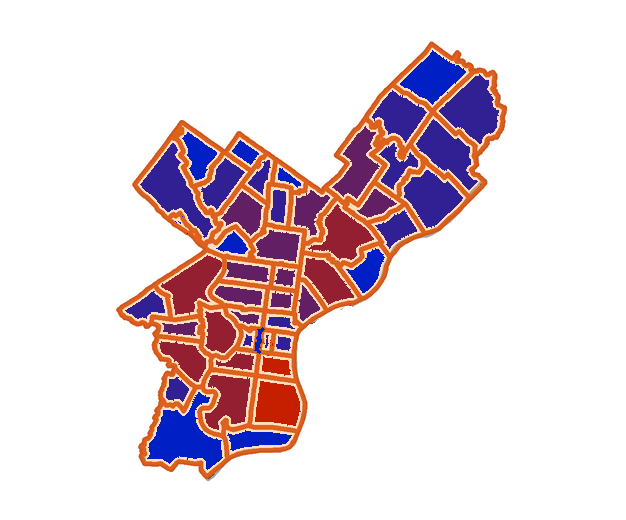
\includegraphics[height=8cm]{graphics/trip-generation.png}
  \caption{Map showing number of fans per zipcode}
  \label{fig-trip-generation-results}
\end{figure}

Looking at the results of the Gravity Model we can tell that ...f

For more accuracy we could include more factors in the model such as
average income of the people living in the zone. We could also use
actual fan data, which we would need to obtain from the Phillies.


\subsection{Trip Distribution}

Trip Distribution data needs to be researched. The SEPTA website has a
Revenue and Ridership Report that gives trip distribution throughout
the day and also average daily ridership, which we can combine and
extrapolate to produce the average number of people riding per minute
throughout the day. Shown below is the trip distribution bar graph
provided in the February 2013 Revenue and Ridership Report:

\begin{figure}[htp]
  \centering
  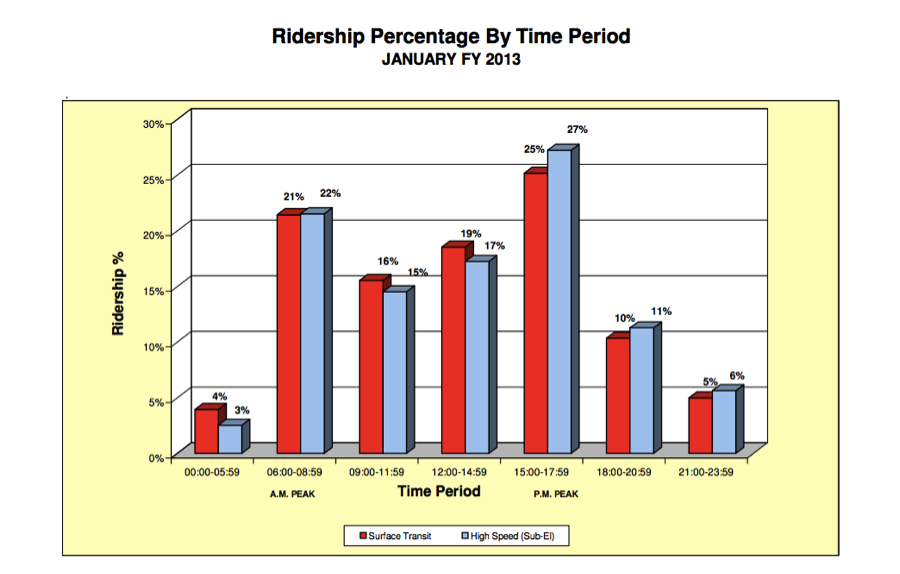
\includegraphics[height=8cm]{graphics/ridership-per-period.png}
  \caption{Average Daily Ridership By Time Period}
  \label{fig-ridership-per-period}
\end{figure}

Furthermore, we used data from a stadium planning study called Traffic
Operations Planning for Stadia and Arenas in order to obtain the
distribution of trips going to a stadium. Below is the table we
obtained:

\begin{table}
  \centering
  \begin{tabular}{cc}
    Minutes to Game Time & Percentage of Crowd \\
    \hline\hline
    -60 minutes & 24\% \\
    -40 minutes & 38\% \\
    -20 minutes & 54\% \\
     Game Time  & 72\% \\
    +20 minutes & 82\% \\
    +40 minutes & 92\% \\
    +60 minutes & 100\% \\
  \end{tabular}
  \caption{Cumulative arrivals to stadium as a percentage of total crowd (45,000 fans)}
  \label{tab-arrivals}
\end{table}

This table gives us the trip distribution for the trips that we
generated from the Trip Generation Gravity Model.


\subsection{Mode Choice}

As we had planned, we were able to obtain both parking lot data from
the Philadelphia Phillies, as well as average ridership data from
SEPTA. We found out that there were on average 7,400 trips per game on
SEPTA. Additionally, we found out there are typically 17,000 cars
parked in the parking lots every game. We found that if back-out the
average number of passengers per car we get 2, which has been
cross-referenced with traffic data for the United States. In order to
back out the number we assume 95\% occupancy of 43,651, or 41,468
total fans. We then removed the number of people taking SEPTA, which
gives us 34,068. Then divide that by the number of cars, which gives
us 2.


\subsection{Trip Assignment}

\subsubsection{SEPTA}

We developed a software module capable of interacting with SEPTA's
data feed, accounting for ``background'' ridership, and routing fans
to the stadium in the most efficient manner possible. The system does
this routing while ensuring now train or bus is filled beyond
capacity, and subject to fan arrival distributions. Once the
large-scale solution has been stored, the system can calculate
incremental changes to demand very quickly, as well as compute summary
statistics for any path. These statistics include:

\begin{itemize}
  \item Total duration
  \item Number of line changes
  \item Expected congestion level across the path
  \item Total waiting time
\end{itemize}

Additionally, we developed a module to map zip codes to SEPTA
stations, which can be combined with the above to present a variety of
travel alternatives to the user.

\subsubsection{Car-Micro}

We developed a simulation capable of reproducing the exiting dynamics
of thousands of cars through a complex network of roads. The
simulation adheres to state-of-the art modeling principles and pushes
the limit on queue-based traffic modeling.

\subsubsection{Support Tools}
As a side-benefit (or prerequisite) of developing these graph-based
simulations, we developed a series of graphical tools for
building and manipulating graphs as well as a Python wrapper for the
popular graph manipulation that will be released as open-source software.

\subsubsection{Car-Macro}

For the long Car model, we were able to utilize the Google Directions
API to retrieve both the distance and time from each zip code defined
in our model to the stadium. The results are stored as comma-separated
values that can be parsed easily from Python. The script needs to be
run two times for each zip code in a given set $Z$, which yields a
runtime of $O(|Z|)$, giving us the distance and time for both modes of
transportation, driving and transit.

Table \ref{tab-zip-dists} shows a table that provides a snippet of the
zip code, distance and time data when using transit to/from the
stadium.

\begin{table}[htp]
  \centering
  \caption{Distance from the stadium by zipcode (excerpt)}
  \label{tab-zip-dists}
  \begin{tabular}{ccc}
    \firsthline
    \bfseries Zipcode & \bfseries Distance & \bfseries Time \\
    & (m) & (min) \\ \hline
    19101 & 6,282 & 22.6 \\
    19102 & 7,048 & 22.6 \\
    19103 & 7,209 & 27.7 \\
    19104 & 9,011 & 28.4 \\
    19105 & 5,311 & 31.3 \\
    19106 & 6,441 & 25.2 \\
    19107 & 5,919 & 35.8 \\
    19108 & 6,356 & 30.7 \\
    19109 & 5,935 & 33.1 \\
    19110 & 5,948 & 22.7 \\
    19111 & 24,602 & 72.0 \\
    19112 & 3,134 & 38.2 \\
    19113 & 14,313 & 31.8 \\
    19114 & 29,006 & 74.4 \\
    19115 & 27,310 & 76.1 \\
    \lasthline
  \end{tabular}
\end{table}

\subsubsection{Transportation and GHG Results}

We were able to source accurate distance and time estimates (as stated
above) for fans traveling from each of the zip codes considered. Our
model then provided estimates for idling time based on congestion
levels and this led us to our first result making a direct comparison
between cars and SEPTA. We obtained was the distribution of travel
time across fans based on the trip generation model. We can see that
close to 12,000 people can save time traveling by SEPTA instead of
taking their car once we account for congestion and idling time in the
stadium. In fact, with only 20 minutes more, close to 40,000 fans can
switch from car to SEPTA, the benefits of which are displayed in our
second comparative result.

\begin{figure}[htp]
  \centering
  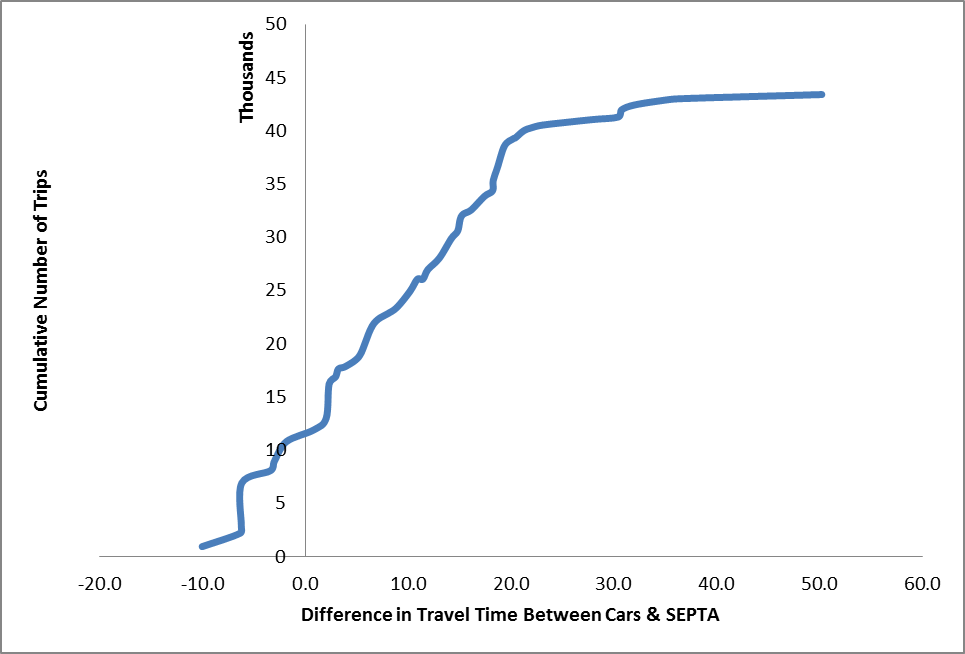
\includegraphics[height=8cm]{graphics/graph1.png}
  \caption{Cumulative number of trips by difference between car and SEPTA travel times}
\end{figure}

We were able to establish accurate estimates for the average
greenhouse gas emissions for both gasoline and diesel cars. We also
sourced estimates for SEPTA train and bus emission per passenger mile
travelled. These estimates were used to compare the relative
environmental tradeoff of choosing cars over public transportation. We
can see that if the aforementioned 12,000 fans switch to SEPTA we
could cut down on approximately 20 million grams of CO2 per one-way
trip to or from a game. If the 40,000 fans identified above were to
switch, hypothetically, even after accounting for SEPTA capacity
constraints and waiting time, we would save close to 80 million grams
of CO2 per one-way trip.

\begin{figure}[htp]
  \centering
  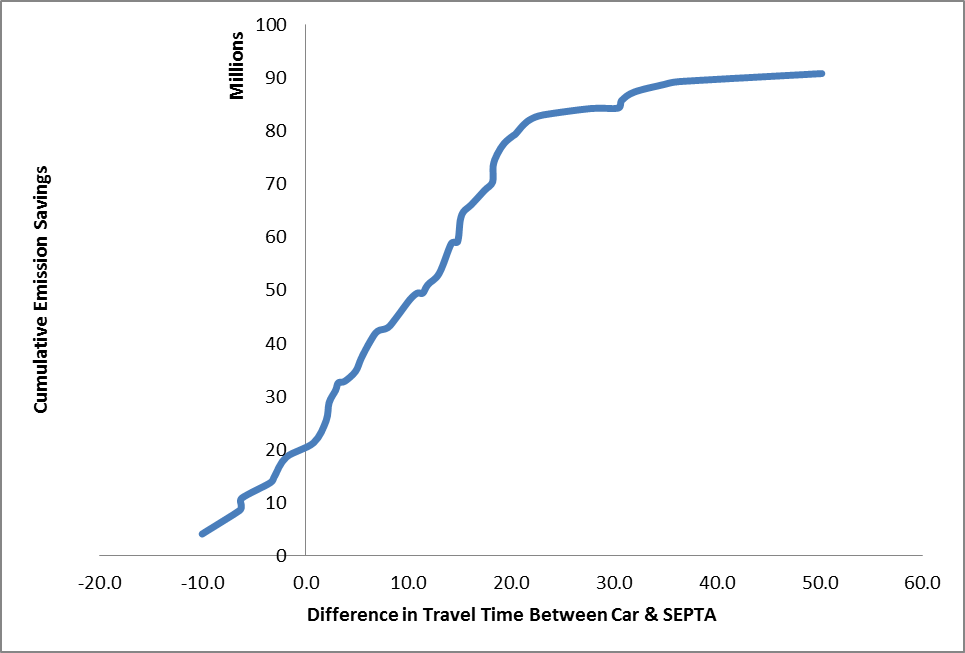
\includegraphics[height=8cm]{graphics/graph2.png}
  \caption{Cumulative carbon emissions by difference between car and SEPTA travel times}
\end{figure}

\subsubsection{Output Results}

As specified in the design, the output was meant to be intuitive,
accessible and impactful. The options we considered were:

\begin{itemize}
    \item Mobile App (iOS, Android, Windows Phone)
    \item Web Application
    \item Desktop Application
\end{itemize}

The design that was settled upon was the second one, Web Application.

Mobile applications have the advantage of being very convenient but
the drawback is that proficiency required across multiple platforms
and programming languages as well as dealing with fragmentation across
versions of mobile operating systems (especially Android) is
especially difficult. Desktop applications suffer from rigidity in
that they are difficult to update on-the-fly and often require tedious
updates via desktop operating systems. As a result, web applications
provide the perfect balance for our project, allowing for updates as
well as accessibility from both desktops and mobile devices.

Once the form of output was finalized, further research was performed
to ensure that we satisfied our goal of having an ``intuitive''
output. Brainstorming was conducted with potential users of the web
application in order to determine the best layout for the information
to be displayed. Basic feedback was also obtained on the overall
aesthetic of the web application. Our basic implementation of the web
application was divided into five pages hosted on a local Python
simple server utilizing CGI scripts to serve webpages in response to
user input.

\begin{description}
    \item[Introduction Page] The introduction page serves as a landing
  page for users of our web application. There is an emission
  calculator, which takes as an input the user's address, zip code and
  vehicle miles per gallon as well as fuel type (gasoline or
  diesel). The page also displays the date and time of the next home
  page as well as the weather within one hour of the start of the game
  in order to allow users to make a more informed decision when
  selecting transportation. Finally, the page provides an overview of
  how the web application works and how emissions are calculated by
  our model.
  \begin{figure}[htp]
    \centering
    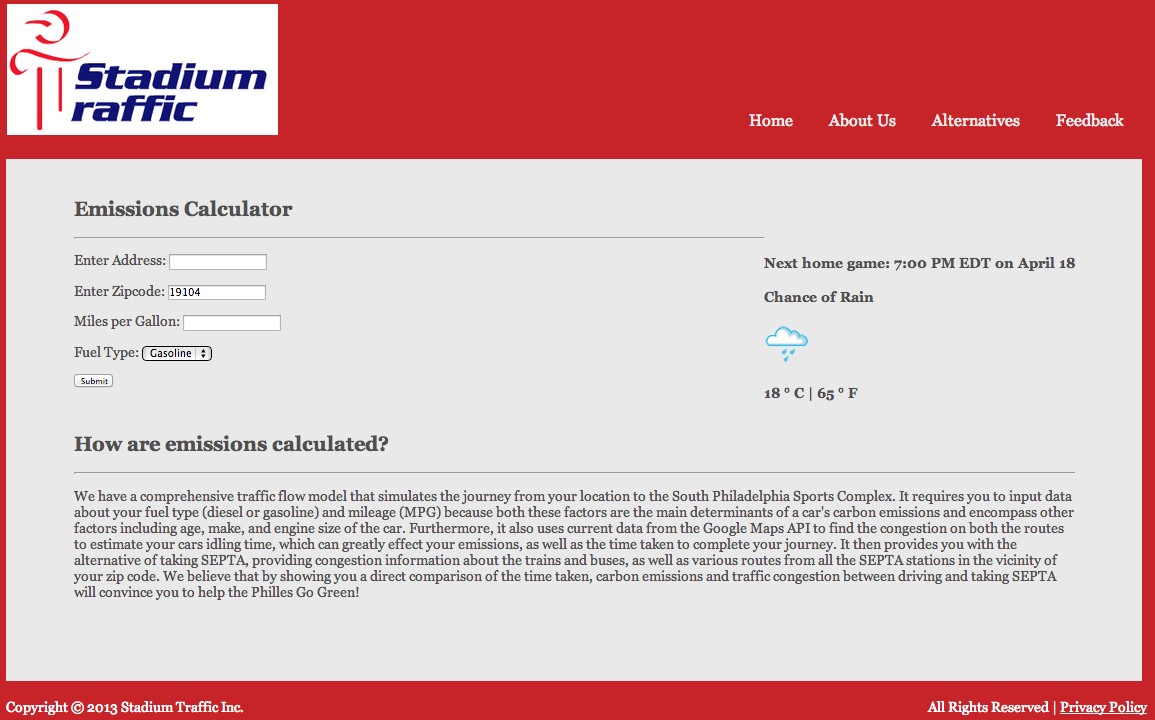
\includegraphics[height=8cm]{graphics/website/intro.png}
    \caption{Introduction Page}
  \end{figure}

    \item[Results Page] The results page is served when the ``submit''
  button on the introduction page is clicked with valid information in
  the form. The results page displays a Google Map showing driving
  directions from the origin to the stadium and provides a drop-down
  to switch to transit directions. The page also provides a
  comparative table between Car and Septa across four factors: time
  taken, distance, carbon emissions and congestion levels. The results
  in the table are driven by the model that we created and serve as
  the main ``output'' of our project.
  \begin{figure}[htp]
    \centering
    \begin{subfigure}{14cm}
      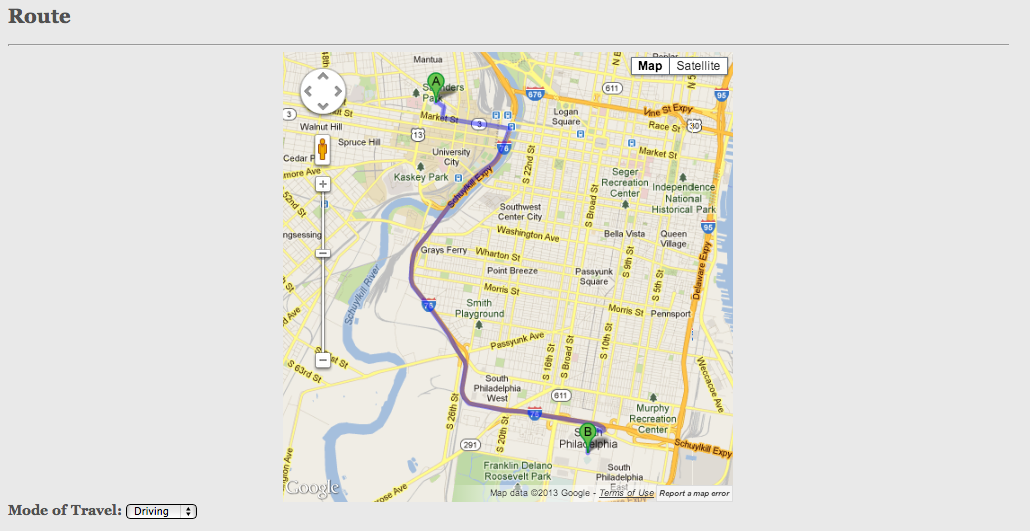
\includegraphics[height=7.22cm]{graphics/website/results-map.png}
      \caption{Results Page (Map)}
    \end{subfigure} \\
    \begin{subfigure}{14cm}
      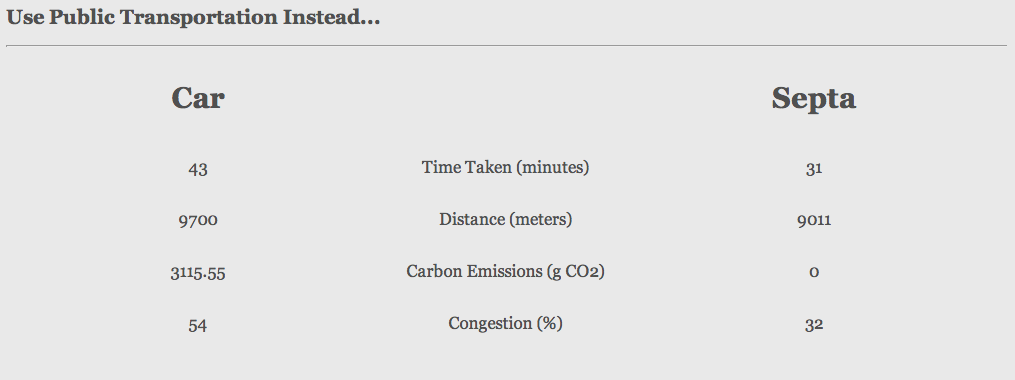
\includegraphics[height=5.24cm]{graphics/website/results-table.png}
      \caption{Results Page (Comparative Table)}
    \end{subfigure}
  \end{figure}

    \item[Alternatives Page] There might be users, however, who prefer
  not to switch to SEPTA. Given that our overall goal was to reduce
  carbon emissions from fans traveling to and from games, we suggest
  two alternatives that fans that utilize to cut down on their carbon
  emissions even if they do opt to take a car to the game. The first
  is to purchase carbon credits from a third-party vendor and the
  other is to utilize a public forum to find other fans to carpool
  with to the next home game.

  \begin{figure}[htp]
    \centering
    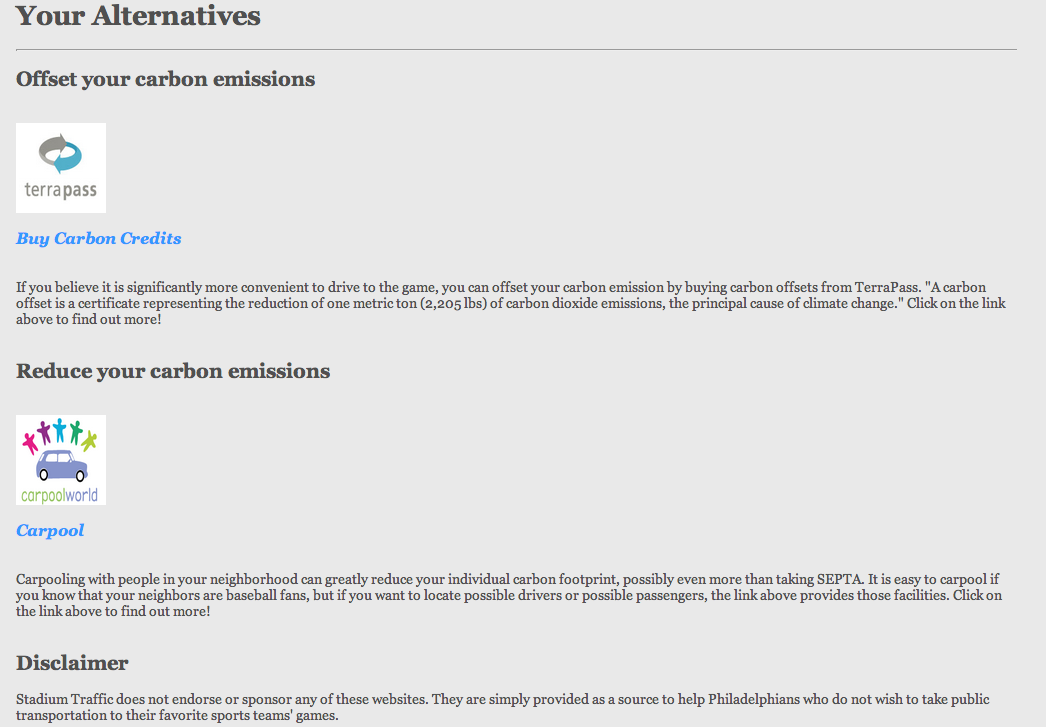
\includegraphics[height=8cm]{graphics/website/alternatives.png}
    \caption{Alternatives Page}
  \end{figure}

    \item[About Page] The about page provides users with information
  about the motivations behind our project and a brief biography for
  each of the three members on our team.

  \begin{figure}[htp]
    \centering
    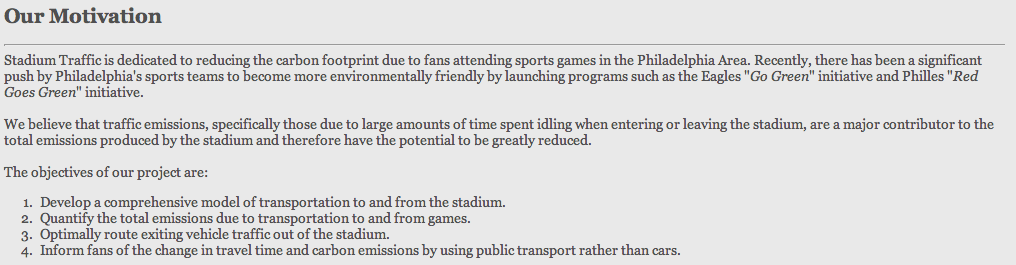
\includegraphics[height=3.65cm]{graphics/website/motivation.png}
    \caption{About Page (Motivation section)}
  \end{figure}

    \item[Feedback Page] The feedback page features a simple form that
  users can utilize to convey compliments/complaints to the Stadium
  Traffic team.

  \begin{figure}[htp]
    \centering
    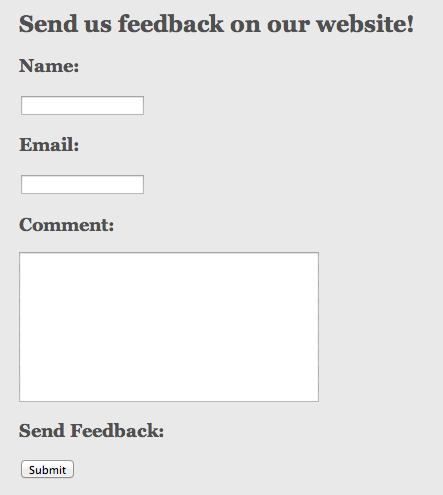
\includegraphics[height=8cm]{graphics/website/feedback.png}
    \caption{Feedback Page}
  \end{figure}
\end{description}

Also, our website contains a privacy policy that was added in order to
inform users about how the information they input will be stored and
utilized as is conventional in most web applications today.


\section{Lessons Learned}

It is important to consistently review and assess your work in order
to derive the maximum benefit from any project and in order to improve
the current and future projects. When conducting a review, one should
not only focus on the mistakes, but also examine what was done well in
order to ensure that it is followed again. Furthermore, one should
analyze the mistakes and understand the underlying reasons that lead
to those mistakes so that they are not made again. Throughout our
project we had review meetings, however at the end it is most
effective when you can look back at the end project and analyze the
project as a whole. As a result of our analysis, below are the main
lessons we learned:

\begin{itemize}
    \item The most important lesson learned was with respect to
  scheduling and particularly the importance of including slack time
  and regularly updating your schedule. We put a lot of effort into
  creating and updating the schedule in order to clearly know how much
  work was left to be done and by what date it had to be completed. By
  not including slack time, when we had setbacks, such as not being
  able to set up a meeting with the Phillies, we fell behind schedule
  and had to do a disproportionately large amount of work towards the
  end. However, we would change the order of tasks to incorporate the
  delays and because we updated our schedule regularly we were always
  aware of our current situation.

    \item It is very important to set deadlines for important
  decisions that can greatly impact your project. We had not set a
  deadline to decide who our end user was because we kept waiting on
  the Phillies to meet us. This decision impacted the model and
  particularly the GUI. If we had set at deadline and chosen earlier,
  we would have had more time to improve our GUI (website) for the
  fans and possibly even been able to launch it.

    \item There is always going to be a tradeoff between runtime and
  accuracy in any simulation and it is important to decide on what is
  the right balance based on your user requirements. This is an
  important decision to make early on so that you can code your model
  accordingly and not have to adjust your model later on.

    \item One thing that helped us greatly was having system block
  diagrams with inputs and outputs of each block clearly
  specified. This enabled us to create each subsystem knowing what
  inputs were available and what outputs had to be produced. This made
  the integration of the system very easy.

    \item Good software documentation and choice of software can make
  your project much easier. Firstly, one software should be chosen at
  the start of the project that everyone is comfortable with because
  when coding is done on multiple software it becomes difficult to
  integrate. Secondly, all code should be excessively documented in
  order to enable team members to work on it together and it also
  makes debugging easier.

    \item It is important and can save you a lot of time if you do a
  thorough search of previous work before you start your project. This
  is because if you find it late you will have redone the work and
  wasted a lot of resources.

\end{itemize}


\section{Equipment/Fabrication/Software Needs}
We do not have any need for specialized equipment or software. The
software we will be using is either publicly available, or available
at Penn. We expect that our production version of the model will not
depend on commercial tools.

\section{Conclusions and Recommendations}

\input{conclusions}

\section{Nomenclature}
{\centering
\midcolumnwidth=.8\textwidth plus 10\tabcolsep minus 10\tabcolsep
\begin{tabular}{%
    >{\raggedright\bfseries}p{.1\textwidth}%
    p{\midcolumnwidth}}
  API & Application programming interface. An official, documented way
  for a program to access a database or another program, such as that
  of Google Maps. \\
  DOM & Document Object Model. A file format that is very easy to
  parse and yet human-readable. \\
  EPP & Emissions per passenger. \\
  EPM & Emissions per mile. \\
  GHG & Greenhouse gases. We mostly mean Carbon Dioxide, but we use
  the term GHG since emissions are highly correlated across types in
  this application. \\
  HBO & Home-based other. A category of trips in the
  standard  model. Contrast with HBS, HBW, NHO, and NHW. \\
  HBS & Home-based shop. A category of trips in the standard
  model. Refers to trips from the home to go shopping. Contrast with
  HBO, HBW, NHO, and NHW. \\
  HBW & Home-based work. A category of trips in the standard
  model. Refers to trips from the home to go to work. Contrast with
  HBO, HBS, NHO, and NHW. \\
  MAG & Maricopa Association of Governments. It is in charge of
  transportation planning for Phoenix and it surroundings. \\
  NHO & Non-home-based other. A category of trips in the standard
  model. Contrast with  HBO, HBS, HBW, and NHW. \\
  NHW & Non-home-based work. A category of trips in the standard
  model. Refers to trips not from the home to go to work. Contrast
  with HBO, HBS, HBW, and NHO. \\
  SEPTA & Southeast Pennsylvania Transit Authority. Manages the
  commuter rail, the subway, trolley, and bus systems in and around
  Philadelphia \\
  SQL & A type of database that is commonly used. \\
  TAZ & Traffic analysis zone. Used in modeling the UTMS. It involves
  dividing a geographical area into units that have sufficiently
  similar transit and demographics to treat as one for the purposes of
  the model. \\
  UTMS & Urban Transportation Modeling System. A commonly used
  framework to model traffic demand and flows. \\
  XML & Extensible markup language. A structured file format that is
  human-readable and easily parseable and customizable. \\
\end{tabular}
}

\makereferences

\makebibliography


\section{Financial Information}
We expect our project to incur minimal cost. At this time, the only
foreseeable expenses are the cost of transportation to the
stadium. Depending on how we refine the user needs after our meeting
with the Eagles, we may have to purchase a mobile device on which to
prototype our model interface.

\section{Ethical Issues}


\subsection{Description of Larger Context}

There are a lot of important stakeholders involved with the project. These include the sports fans who are the potential end users and will input personal data into the system and receive outputs, the sports teams (Philadelphia Phillies, Eagles and Flyers) who are undertaking initiatives with similar goals and SEPTA who will have more passengers if our project is a success.


\subsection{Analysis of Ethical Issues}

There are a number of ethical issues that may arise when our project is launched to the public. The first obvious issue arises with the conflict of interest with the parking lots. If more people take SEPTA then it will reduce their revenue and they would not be happy with it and may even have to charge higher prices to the people who continue to drive. Item 2 in the IEEE Code of Ethics says “to avoid real or perceived conflicts of interest whenever possible, and to disclose them to affected parties when they do exist;” and even the INCOSE Code of Ethics says “Avoid conflicts of interest and the appearance thereof.” Since we are affecting their business, we are harming them, which is in conflict with the ACM Code of Ethics section 1.2 Avoid harm to others. Furthermore, it may even be a conflict of interest with the sports teams and other food or merchandise vendors who make money when people tailgate and promote the experience, because if people don’t drive then they can’t tailgate. The above sections of all three codes of ethics are also relevant to this.

Another concern may arise because of the links to other websites for carpooling and buying carbon offsets. If there is any legal issues that arise from the misconduct websites, we do not want to be held liable so it is important to have a disclaimer that is clearly visible and explicitly states that we are not affiliated with those websites in anyway. One potential legal issue would be if it is found out that the carbon offsets website is misusing the donations. This could transfer over to us if we are known to be affiliated with them, so we need to make sure we are not.  A similar liability could arise from the carpool website if there were any security lapses that arise. That is why it is important to make sure that we have no legal connection with them and make that clear on our website. This would also be in line with the IEEE first code of conduct that states “to accept responsibility in making decisions consistent with the safety, health, and welfare of the public, and to disclose promptly factors that might endanger the public or the environment” and the INCOSE code that states “Accept responsibility for your actions and engineering results, including being open to ethical scrutiny and assessment.”

Misleading our users has some ethical ramifications that is why it should be clear what information we are providing and how it was calculated. Two areas that could be potentially misleading are providing zero carbon emissions from SEPTA on the website, which we have to make clear are the marginal emissions because the train will be running anyways. It would be wrong to make the user believe that SEPTA produces no emissions. The other area that could be misleading is when we provide an approximate driving and SEPTA travel time, because this is based on data from a simulation for an average car and the time may vary greatly for any specific car depending on where exactly they park. Therefore this must be made clear. These are in line with the IEEE Code of Conduct sections 3 and 6 that state “to be honest and realistic in stating claims or estimates based on available data” and “to maintain and improve our technical competence and to undertake technological tasks for others only if qualified by training or experience, or after full disclosure of pertinent limitations” respectively. Even the following INCOSE Code of Ethics items are relevant: “Act legally, honorably, honestly, justly, and responsibly” and “Give prudent advice. Be truthful, objective, and maintain your professional and technical integrity.”

We should also make sure to attribute Google for the data that we get from Google Maps API because the ACM Code of Ethics section 1.6 says that we should “Give proper credit for intellectual property.”

\subsection{Recommendations}

The most pressing concerns are those of the legal liability from third party websites and the conflict of interest with the parking lot owners. There are possible legal or market-based solutions. We could have disclaimers showing no affiliation with the websites and do our own due diligence on any websites that we provide links to. For the conflict of interest, we could consult a lawyer to make sure that no legal action can be taken against us by the parking lot operators if their sales are affected. We could also work together with the parking lot to provide them with other sources of income such as organization of tailgating services for people who take SEPTA and don’t have cars. We could also work with the sports teams to get compensation for helping them reduce traffic and achieve their goals of becoming more environmentally friendly and split some of that remuneration with the parking lot operators. Finally, the last ethical concern arising from misleading users can be easily mitigated by clearly stating our method and assumptions used to calculate the output. This way the user would be informed and not misunderstand anything.


\appendix

\section{A Documented Module of Code}
\lstinputlisting[language=python,basicstyle=\small]{includes/module.py}
\end{document}

%  LocalWords:  DOM EPP EPM GHG Huemmler Vukan Vuchic ITE
